\documentclass{standalone}
\usepackage{tikz}
\usetikzlibrary{patterns, positioning}
\usepackage[sfdefault]{ClearSans} %% option 'sfdefault' activates Clear Sans as the default text font
\usepackage[T1]{fontenc}

\begin{document}
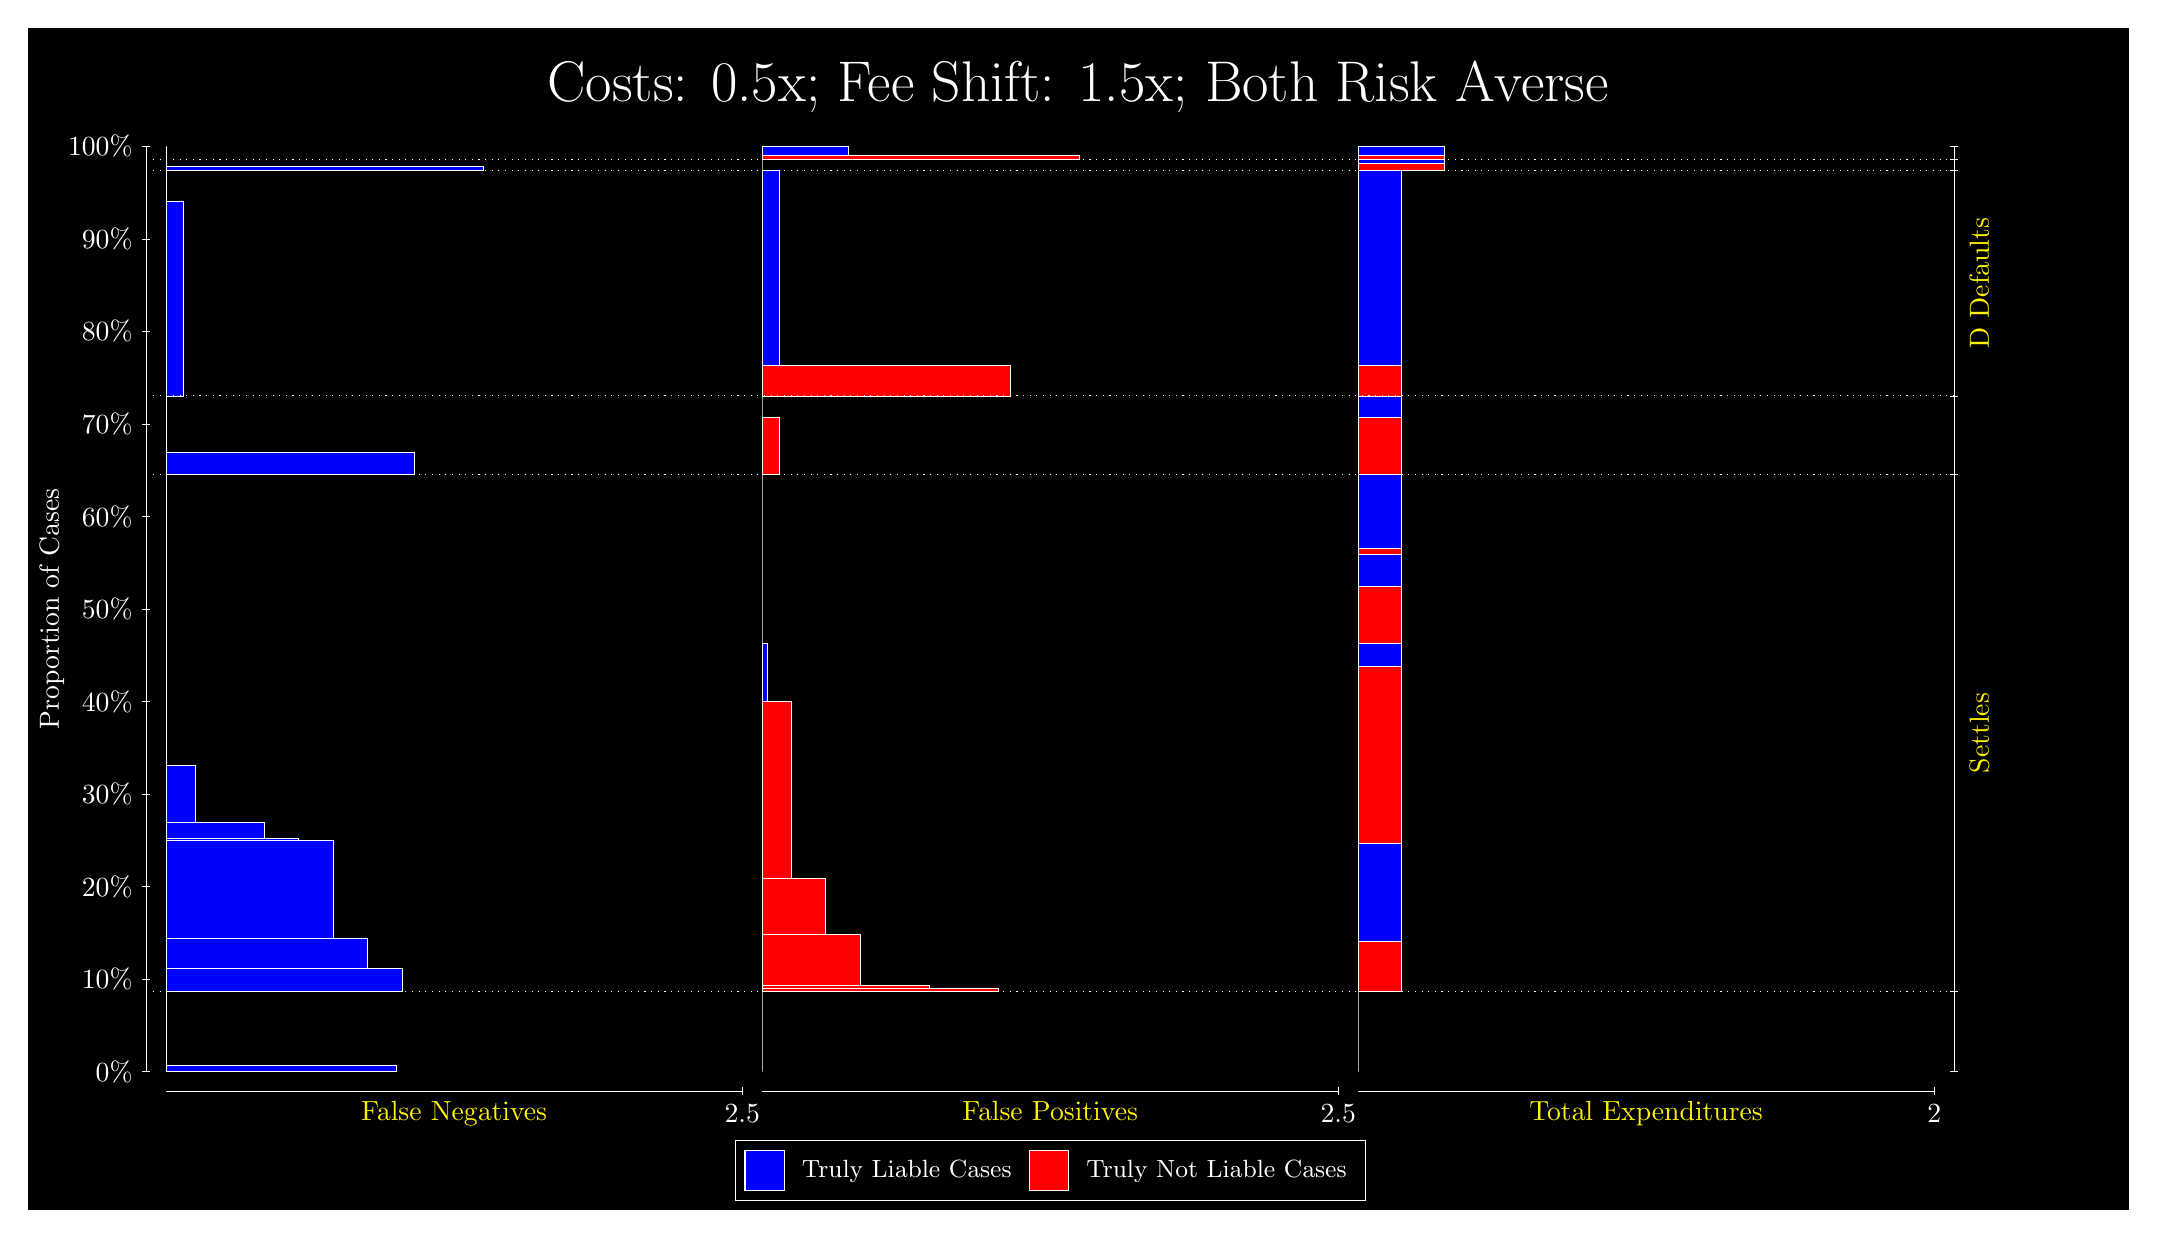
\begin{tikzpicture}
\draw[fill=black] (0,0) rectangle (26.667,15);
\draw[text=white] (0,13.5) rectangle (26.667,15) node[midway] {\huge Costs: 0.5x; Fee Shift: 1.5x; Both Risk Averse};
\draw[white, very thin] (1.5,1.75) -- (1.5,13.5);
\node[rotate=90, text=white, anchor=center] at (0.3, 7.625) {Proportion of Cases};
\draw[white, very thin] (1.45,1.75) -- (1.55,1.75);
\node[text=white, anchor=east] at (1.45, 1.75) {0\%};
\draw[white, very thin] (1.45,2.925) -- (1.55,2.925);
\node[text=white, anchor=east] at (1.45, 2.925) {10\%};
\draw[white, very thin] (1.45,4.1) -- (1.55,4.1);
\node[text=white, anchor=east] at (1.45, 4.1) {20\%};
\draw[white, very thin] (1.45,5.275) -- (1.55,5.275);
\node[text=white, anchor=east] at (1.45, 5.275) {30\%};
\draw[white, very thin] (1.45,6.45) -- (1.55,6.45);
\node[text=white, anchor=east] at (1.45, 6.45) {40\%};
\draw[white, very thin] (1.45,7.625) -- (1.55,7.625);
\node[text=white, anchor=east] at (1.45, 7.625) {50\%};
\draw[white, very thin] (1.45,8.8) -- (1.55,8.8);
\node[text=white, anchor=east] at (1.45, 8.8) {60\%};
\draw[white, very thin] (1.45,9.975) -- (1.55,9.975);
\node[text=white, anchor=east] at (1.45, 9.975) {70\%};
\draw[white, very thin] (1.45,11.15) -- (1.55,11.15);
\node[text=white, anchor=east] at (1.45, 11.15) {80\%};
\draw[white, very thin] (1.45,12.325) -- (1.55,12.325);
\node[text=white, anchor=east] at (1.45, 12.325) {90\%};
\draw[white, very thin] (1.45,13.5) -- (1.55,13.5);
\node[text=white, anchor=east] at (1.45, 13.5) {100\%};

\draw[white, very thin] (24.457,1.75) -- (24.457,13.5);
\draw[white, very thin] (24.407,1.75) -- (24.507,1.75);
\node[anchor=west] at (24.407, 1.75) {};
\draw[white, very thin] (24.407,2.7636) -- (24.507,2.7636);
\node[anchor=west] at (24.407, 2.7636) {};
\draw[white, very thin] (24.407,9.3332) -- (24.507,9.3332);
\node[anchor=west] at (24.407, 9.3332) {};
\draw[white, very thin] (24.407,10.33) -- (24.507,10.33);
\node[anchor=west] at (24.407, 10.33) {};
\draw[white, very thin] (24.407,13.192) -- (24.507,13.192);
\node[anchor=west] at (24.407, 13.192) {};
\draw[white, very thin] (24.407,13.334) -- (24.507,13.334);
\node[anchor=west] at (24.407, 13.334) {};
\draw[white, very thin] (24.407,13.5) -- (24.507,13.5);
\node[anchor=west] at (24.407, 13.5) {};

\draw[white, very thin, fill=blue] (1.75,1.75) rectangle (4.6775,1.832);
\draw[white, very thin, fill=red] (1.75,1.832) rectangle (1.75,2.7636);
\draw[white, very thin, fill=blue] (1.75,2.7636) rectangle (4.7507,3.0555);
\draw[white, very thin, fill=blue] (1.75,3.0555) rectangle (4.3116,3.4447);
\draw[white, very thin, fill=blue] (1.75,3.4447) rectangle (3.8725,4.6851);
\draw[white, very thin, fill=blue] (1.75,4.6851) rectangle (3.4333,4.7102);
\draw[white, very thin, fill=blue] (1.75,4.7102) rectangle (2.9942,4.9129);
\draw[white, very thin, fill=blue] (1.75,4.9129) rectangle (2.1159,5.6434);
\draw[white, very thin, fill=red] (1.75,5.6434) rectangle (1.75,9.3332);
\draw[white, very thin, fill=blue] (1.75,9.3332) rectangle (4.8971,9.61);
\draw[white, very thin, fill=red] (1.75,9.61) rectangle (1.75,10.33);
\draw[white, very thin, fill=blue] (1.75,10.33) rectangle (1.9696,12.801);
\draw[white, very thin, fill=red] (1.75,12.801) rectangle (1.75,13.192);
\draw[white, very thin, fill=blue] (1.75,13.192) rectangle (5.7754,13.246);
\draw[white, very thin, fill=red] (1.75,13.246) rectangle (1.75,13.334);
\draw[white, very thin, fill=red] (1.75,13.334) rectangle (1.75,13.388);
\draw[white, very thin, fill=blue] (1.75,13.388) rectangle (1.75,13.5);
\draw[white, very thin, fill=red] (9.3189,1.75) rectangle (9.3189,2.6815);
\draw[white, very thin, fill=blue] (9.3189,2.6815) rectangle (9.3189,2.7636);
\draw[white, very thin, fill=red] (9.3189,2.7636) rectangle (12.32,2.8109);
\draw[white, very thin, fill=red] (9.3189,2.8109) rectangle (11.441,2.8392);
\draw[white, very thin, fill=red] (9.3189,2.8392) rectangle (11.002,2.8486);
\draw[white, very thin, fill=red] (9.3189,2.8486) rectangle (10.563,3.4913);
\draw[white, very thin, fill=red] (9.3189,3.4913) rectangle (10.124,4.2055);
\draw[white, very thin, fill=red] (9.3189,4.2055) rectangle (9.6848,6.4534);
\draw[white, very thin, fill=blue] (9.3189,6.4534) rectangle (9.3921,7.1839);
\draw[white, very thin, fill=blue] (9.3189,7.1839) rectangle (9.3189,9.3332);
\draw[white, very thin, fill=red] (9.3189,9.3332) rectangle (9.5384,10.054);
\draw[white, very thin, fill=blue] (9.3189,10.054) rectangle (9.3189,10.33);
\draw[white, very thin, fill=red] (9.3189,10.33) rectangle (12.466,10.721);
\draw[white, very thin, fill=blue] (9.3189,10.721) rectangle (9.5384,13.192);
\draw[white, very thin, fill=red] (9.3189,13.192) rectangle (9.3189,13.281);
\draw[white, very thin, fill=blue] (9.3189,13.281) rectangle (9.3189,13.334);
\draw[white, very thin, fill=red] (9.3189,13.334) rectangle (13.344,13.388);
\draw[white, very thin, fill=blue] (9.3189,13.388) rectangle (10.417,13.5);
\draw[white, very thin, fill=red] (16.888,1.75) rectangle (16.888,2.6815);
\draw[white, very thin, fill=blue] (16.888,2.6815) rectangle (16.888,2.7636);
\draw[white, very thin, fill=red] (16.888,2.7636) rectangle (17.437,3.4063);
\draw[white, very thin, fill=blue] (16.888,3.4063) rectangle (17.437,4.6466);
\draw[white, very thin, fill=red] (16.888,4.6466) rectangle (17.437,6.8945);
\draw[white, very thin, fill=blue] (16.888,6.8945) rectangle (17.437,7.1865);
\draw[white, very thin, fill=red] (16.888,7.1865) rectangle (17.437,7.91);
\draw[white, very thin, fill=blue] (16.888,7.91) rectangle (17.437,8.3244);
\draw[white, very thin, fill=red] (16.888,8.3244) rectangle (17.437,8.4);
\draw[white, very thin, fill=blue] (16.888,8.4) rectangle (17.437,9.3332);
\draw[white, very thin, fill=red] (16.888,9.3332) rectangle (17.437,10.054);
\draw[white, very thin, fill=blue] (16.888,10.054) rectangle (17.437,10.33);
\draw[white, very thin, fill=red] (16.888,10.33) rectangle (17.437,10.721);
\draw[white, very thin, fill=blue] (16.888,10.721) rectangle (17.437,13.192);
\draw[white, very thin, fill=red] (16.888,13.192) rectangle (17.986,13.281);
\draw[white, very thin, fill=blue] (16.888,13.281) rectangle (17.986,13.334);
\draw[white, very thin, fill=red] (16.888,13.334) rectangle (17.986,13.388);
\draw[white, very thin, fill=blue] (16.888,13.388) rectangle (17.986,13.5);
\draw[white, dotted] (1.5,2.7636) -- (24.457,2.7636);
\draw[white, dotted] (1.5,9.3332) -- (24.457,9.3332);
\draw[white, dotted] (1.5,10.33) -- (24.457,10.33);
\draw[white, dotted] (1.5,13.192) -- (24.457,13.192);
\draw[white, dotted] (1.5,13.334) -- (24.457,13.334);
\draw[white, very thin] (1.75,1.5) -- (9.0689,1.5);
\node[text=yellow, anchor=north] at (5.4094, 1.5) {False Negatives};
\draw[white, very thin] (9.0689,1.45) -- (9.0689,1.55);
\node[text=white, anchor=north] at (9.0689, 1.45) {2.5};

\draw[white, very thin] (9.3189,1.5) -- (16.638,1.5);
\node[text=yellow, anchor=north] at (12.978, 1.5) {False Positives};
\draw[white, very thin] (16.638,1.45) -- (16.638,1.55);
\node[text=white, anchor=north] at (16.638, 1.45) {2.5};

\draw[white, very thin] (16.888,1.5) -- (24.207,1.5);
\node[text=yellow, anchor=north] at (20.547, 1.5) {Total Expenditures};
\draw[white, very thin] (24.207,1.45) -- (24.207,1.55);
\node[text=white, anchor=north] at (24.207, 1.45) {2};


\node[text=yellow, centered, rotate=90] at (24.777, 6.0484) {Settles};

\node[text=yellow, centered, rotate=90] at (24.777, 11.761) {D Defaults};



\draw (12.978300999999998,1.5) node[draw=none] (baseCoordinate) {};
\begin{scope}[align=center]
        \matrix[scale=0.5, draw=white, below=0.5cm of baseCoordinate, nodes={draw}, column sep=0.1cm]{
            \node[rectangle, draw, minimum width=0.5cm, minimum height=0.5cm, fill=blue] {}; &
            \node[draw=none, font=\small, text=white] (B) {Truly Liable Cases}; &
            \node[rectangle, draw, minimum width=0.5cm, minimum height=0.5cm, fill=red] {}; &
            \node[draw=none, font=\small, text=white] (B) {Truly Not Liable Cases}; \\
            };
\end{scope}

\end{tikzpicture}
\end{document}